% Revised manuscript. Prior version is preserved in backups/.
% Empirical values come from the repository-generated numbers.tex and tables/.
% Bibliographic keys follow the research repository. See audit/ for checks.
\documentclass[11pt]{article}
\usepackage[margin=1in]{geometry}
\usepackage[T1]{fontenc}
\usepackage[utf8]{inputenc}
\usepackage{lmodern,microtype}
\usepackage{booktabs,graphicx,amsmath,amssymb,array,tabularx}
\usepackage{xcolor,enumitem,caption,placeins,adjustbox,etoolbox}
\usepackage[numbers,sort&compress]{natbib}
\usepackage[hidelinks]{hyperref}
\usepackage{xurl}
% Generated by manuscript/make_numbers.py from logged results. Do not edit by hand.
\newcommand{\AuditBudget}{1}
\newcommand{\AuditExposed}{9}
\newcommand{\AuditExposedHi}{68.3}
\newcommand{\AuditExposedLo}{27.3}
\newcommand{\AuditExposedPct}{47.4}
\newcommand{\AuditFixedK}{12}
\newcommand{\AuditN}{19}
\newcommand{\AuditUncertainty}{3}
\newcommand{\EoneNq}{9,253}
\newcommand{\EoneNqCovidqa}{1,771}
\newcommand{\EoneNqCuad}{996}
\newcommand{\EoneNqQasper}{1,742}
\newcommand{\EoneNqSquadtwo}{4,744}
\newcommand{\EtwoEmFiveTwelveBudget}{0.125}
\newcommand{\EtwoEmFiveTwelveCount}{0.090}
\newcommand{\EtwoEmOneTwoEightBudget}{0.085}
\newcommand{\EtwoEmOneTwoEightCount}{0.105}
\newcommand{\EtwoJobsCuad}{400}
\newcommand{\EtwoJobsQasper}{400}
\newcommand{\EtwoPoneCov}{+0.089}
\newcommand{\EtwoPoneCovHi}{+0.132}
\newcommand{\EtwoPoneCovLo}{+0.050}
\newcommand{\EtwoPoneCovMde}{0.059}
\newcommand{\EtwoPoneEm}{\ensuremath{-}0.055}
\newcommand{\EtwoPoneEmHi}{\ensuremath{-}0.010}
\newcommand{\EtwoPoneEmLo}{\ensuremath{-}0.100}
\newcommand{\EtwoPoneEmMde}{0.066}
\newcommand{\EtwoPoneFone}{\ensuremath{-}0.017}
\newcommand{\EtwoPoneFoneHi}{+0.033}
\newcommand{\EtwoPoneFoneLo}{\ensuremath{-}0.065}
\newcommand{\EtwoPoneFoneMde}{0.068}
\newcommand{\EtwoPoneFoneMdeStrat}{0.068}
\newcommand{\EtwoSquadFiveTwelveBudgetCov}{0.88}
\newcommand{\EtwoSquadFiveTwelveBudgetFone}{0.58}
\newcommand{\EtwoSquadOneTwoEightBudgetCov}{0.86}
\newcommand{\EtwoSquadOneTwoEightBudgetFone}{0.44}
\newcommand{\EtwoSthreeCov}{+0.035}
\newcommand{\EtwoSthreeCovHi}{+0.060}
\newcommand{\EtwoSthreeCovLo}{+0.015}
\newcommand{\EtwoSthreeCovMde}{0.036}
\newcommand{\EtwoSthreeEm}{\ensuremath{-}0.015}
\newcommand{\EtwoSthreeEmHi}{+0.020}
\newcommand{\EtwoSthreeEmLo}{\ensuremath{-}0.050}
\newcommand{\EtwoSthreeEmMde}{0.051}
\newcommand{\EtwoSthreeFone}{+0.004}
\newcommand{\EtwoSthreeFoneHi}{+0.036}
\newcommand{\EtwoSthreeFoneLo}{\ensuremath{-}0.024}
\newcommand{\EtwoSthreeFoneMde}{0.044}
\newcommand{\EtwoTruncCuad}{65}
\newcommand{\EtwoTruncQasper}{2}
\newcommand{\HFiveBBudget}{91.7}
\newcommand{\HFiveBCount}{33.3}
\newcommand{\HFiveBEst}{58.3}
\newcommand{\HFiveBHi}{64.6}
\newcommand{\HFiveBLo}{45.1}
\newcommand{\HFiveBVerdict}{supported}
\newcommand{\HFiveBudgetFiveTwelve}{5.6}
\newcommand{\HFiveCountFiveTwelve}{25.0}
\newcommand{\HFiveEst}{19.4}
\newcommand{\HFiveHi}{41.7}
\newcommand{\HFiveLo}{16.7}
\newcommand{\HFiveSeedMax}{24.3}
\newcommand{\HFiveSeedMin}{21.5}
\newcommand{\HFiveSeedN}{9}
\newcommand{\HFiveVerdict}{inconclusive}
\newcommand{\HFourBBudget}{71.3}
\newcommand{\HFourBCount}{6.9}
\newcommand{\HFourBEst}{64.4}
\newcommand{\HFourBHi}{68.3}
\newcommand{\HFourBLo}{56.5}
\newcommand{\HFourBVerdict}{supported}
\newcommand{\HFourBmOnlyBudget}{61.1}
\newcommand{\HFourBmOnlyCount}{0.0}
\newcommand{\HFourBmOnlyEst}{61.1}
\newcommand{\HFourBmOnlyHi}{72.5}
\newcommand{\HFourBmOnlyLo}{57.2}
\newcommand{\HFourBudget}{64.8}
\newcommand{\HFourCount}{9.4}
\newcommand{\HFourDenseOnlyBudget}{68.5}
\newcommand{\HFourDenseOnlyCount}{18.8}
\newcommand{\HFourDenseOnlyEst}{49.8}
\newcommand{\HFourDenseOnlyHi}{58.1}
\newcommand{\HFourDenseOnlyLo}{39.1}
\newcommand{\HFourEst}{55.4}
\newcommand{\HFourHi}{63.1}
\newcommand{\HFourLo}{50.8}
\newcommand{\HFourVerdict}{supported}
\newcommand{\HOneBEst}{26.7}
\newcommand{\HOneBHi}{33.9}
\newcommand{\HOneBLo}{15.4}
\newcommand{\HOneBVerdict}{supported}
\newcommand{\HOneEst}{71.1}
\newcommand{\HOneHi}{81.9}
\newcommand{\HOneLo}{64.8}
\newcommand{\HOneVerdict}{supported}
\newcommand{\HThreeMedianN}{1,256}
\newcommand{\HThreeShare}{85.4}
\newcommand{\HThreeVerdict}{supported}
\newcommand{\HTwoDatasetEta}{0.61}
\newcommand{\HTwoFraction}{100.0}
\newcommand{\HTwoRetrieverEta}{0.04}
\newcommand{\HTwoVerdict}{supported}
\newcommand{\PoneBudgetFiveTwelve}{7.6}
\newcommand{\PoneBudgetOneTwoEight}{81.2}
\newcommand{\PoneCountFiveTwelve}{78.8}
\newcommand{\PoneCountOneTwoEight}{0.0}
\newcommand{\PoneDenseUniversesBudget}{36}
\newcommand{\PoneDenseUniversesCount}{48}
\newcommand{\PoneUniversesBudget}{576}
\newcommand{\PoneUniversesCount}{768}
\newcommand{\PosthocCharFlips}{965}
\newcommand{\PosthocEquivElements}{85,275,648}
\newcommand{\PosthocEquivElementsB}{1,665,540}
\newcommand{\PosthocUniverses}{24,960}
\newcommand{\SemBpMax}{320}
\newcommand{\SemBpMin}{278}
\newcommand{\SemClMax}{458}
\newcommand{\SemClMin}{452}
\newcommand{\SemClNoncontigMin}{92.0}
\newcommand{\SensAllBudgetsEst}{74.2}
\newcommand{\SensAllBudgetsHi}{84.8}
\newcommand{\SensAllBudgetsLo}{68.3}
\newcommand{\SensBHEst}{68.0}
\newcommand{\SensBHPooledEst}{70.4}
\newcommand{\SensClusterEst}{69.7}
\newcommand{\SensClusterHi}{82.0}
\newcommand{\SensClusterLo}{63.8}
\newcommand{\SensDefRetEst}{70.8}
\newcommand{\SensDefRetHi}{85.4}
\newcommand{\SensDefRetLo}{64.6}
\newcommand{\SensNoSquadEst}{61.5}
\newcommand{\SensNoSquadHi}{74.8}
\newcommand{\SensNoSquadLo}{53.2}
\newcommand{\SfiveOneTwoEightBudgetFix}{75.0}
\newcommand{\SfiveOneTwoEightBudgetSem}{8.3}
\newcommand{\SfiveOneTwoEightCountFix}{16.7}
\newcommand{\SfiveOneTwoEightCountSem}{60.4}
\newcommand{\SfiveUniversesBudget}{72}
\newcommand{\SfiveUniversesCount}{96}
\newcommand{\SoneOneTwoEightBudgetA}{60.5}
\newcommand{\SoneOneTwoEightBudgetB}{6.2}
\newcommand{\SoneOneTwoEightCountA}{0.0}
\newcommand{\SoneOneTwoEightCountB}{74.1}
\newcommand{\SoneSixFourBudgetA}{20.0}
\newcommand{\SoneSixFourBudgetB}{42.1}
\newcommand{\SoneSixFourCountB}{84.1}
\newcommand{\StwoOneTwoEightBudgetA}{55.1}
\newcommand{\StwoOneTwoEightBudgetB}{1.9}
\newcommand{\StwoOneTwoEightCountA}{51.6}
\newcommand{\StwoOneTwoEightCountB}{1.8}
\newcommand{\StwoTwoFiveSixBudgetA}{39.8}
\newcommand{\StwoTwoFiveSixBudgetB}{3.3}
\newcommand{\StwoTwoFiveSixCountA}{36.1}
\newcommand{\StwoTwoFiveSixCountB}{3.5}

\newcommand{\pp}{\ensuremath{\,\mathrm{pp}}}
\newcommand{\chunk}[1]{\texttt{#1}}
\newcommand{\ind}{\mathbb{1}}
% Compatibility with the repository's generated audit table.
% Bibliographic identity checks and full-text checks are logged separately.
\newcommand{\citeL}[1]{\cite{#1}}
\newcommand{\AuthorName}{}
\newcommand{\AuthorAffiliation}{}
\newcommand{\AuthorEmail}{}
\captionsetup{font=small,labelfont=bf,skip=6pt}
\setlength{\emergencystretch}{2em}
\setlength{\tabcolsep}{3pt}
\setlist{nosep}
\renewcommand{\bibfont}{\small}
\setlength{\bibsep}{3pt}
\renewcommand{\topfraction}{0.92}
\renewcommand{\bottomfraction}{0.85}
\renewcommand{\textfraction}{0.08}
\renewcommand{\floatpagefraction}{0.75}
\setcounter{topnumber}{3}
\setcounter{totalnumber}{5}
% Fit generated tables without editing their numerical contents or filenames.
\BeforeBeginEnvironment{tabular}{\begin{adjustbox}{max width=\linewidth}}
\AfterEndEnvironment{tabular}{\end{adjustbox}}
% This manuscript is single-column. Permit generated [t] tables to sit here
% as well as at a page boundary, without changing the generated source files.
\let\RepoTable\table
\let\EndRepoTable\endtable
\renewenvironment{table}[1][htbp]{\RepoTable[htbp]}{\EndRepoTable}
\renewenvironment{table*}[1][htbp]{\RepoTable[htbp]}{\EndRepoTable}

\hypersetup{pdftitle={Chunking Verdicts in Retrieval-Augmented Generation Depend on the Evaluation Protocol: A Pre-registered Multiverse Analysis},pdfsubject={Pre-registered analysis of chunking evaluation protocols}}
\title{Chunking Verdicts in Retrieval-Augmented Generation Depend on the Evaluation Protocol:\texorpdfstring{\\}{ }A Pre-registered Multiverse Analysis}
\author{\AuthorName}
\date{}
\makeatletter
\renewcommand{\@maketitle}{%
  \begin{center}
    {\LARGE \@title\par}
    \ifx\AuthorName\@empty\else
      \vskip 0.8em {\large \AuthorName\par}
      \AuthorAffiliation\par\texttt{\AuthorEmail}\par
    \fi
  \end{center}
  \vskip 0.8em
}
\makeatother
\begin{document}
\maketitle

\begin{abstract}
Comparisons of chunking strategies in retrieval-augmented generation can fix the number of retrieved passages while allowing their total length to vary. Coverage-based metrics may then reward the extra text rather than better segmentation. We examine this dependence in two pre-registered multiverse studies across four English question-answering datasets and \EoneNq{} held-out queries. Matching retrieval by word budget rather than chunk count reduces support for 512-word over 128-word chunks by \HOneEst{} percentage points (95\% CI [\HOneLo, \HOneHi]). In semantic-breakpoint comparisons, support for the shorter arm rises by \HFourEst{} points ([\HFourLo, \HFourHi]). Semantic clustering and dense retrieval also show protocol sensitivity, although the original dense-retrieval hypothesis is inconclusive. An exploratory Qwen3-4B evaluation finds positive retrieval-coverage contrasts but no corresponding positive answer-F1 interaction. The results show why a chunking preference must be tied to its operating constraint. We recommend reporting both retrieval depth and retrieved-text budget, and evaluating answer quality separately.
\end{abstract}

\section{Introduction}
Retrieval-augmented generation (RAG) combines a language model with material retrieved from a document collection~\cite{lewis2020rag,gao2023ragsurvey}. Chunking determines which parts of that collection can be ranked and passed to the model. A useful comparison of chunkers must therefore answer two questions: what changes between the systems, and what remains fixed?

Consider two systems that each retrieve five passages. One uses a cap of 128 words per chunk; the other uses 512. Equal retrieval depth gives the second system a much larger potential text allowance. A metric that asks whether retrieved text contains a gold evidence span can reward that allowance, even when the longer chunks are not ranked more precisely. Matching the retrieved word budget removes this difference, but also changes the number of passages and can truncate the last selected chunk. The two protocols evaluate different operating conditions.

We ask how strongly this choice affects the direction and statistical support of a chunking comparison. Rather than choose one dataset, retriever and retrieval depth, we evaluate a declared grid of settings through a multiverse analysis~\cite{steegen2016multiverse}. Each setting, or \emph{universe}, produces a paired comparison between two chunkers. We summarize the share of universes supporting each arm under count-matched and word-budget-matched selection.

The primary comparison is between \chunk{fixed-128} and \chunk{fixed-512}. Support for the larger arm falls by \HOneEst\pp{} under budget matching. The overlap comparisons change much less, while paragraph and semantic chunkers show substantial sensitivity when their realized lengths differ from those of the fixed windows. A dense-retrieval extension shows that the starting preference also depends on the retriever. Finally, an answer-generation experiment tests whether the retrieval pattern carries over to the end task.

Our contribution is an estimate of protocol sensitivity across two pre-registered studies, together with an answer-level check that establishes the limits of the retrieval result. A provisional audit of recent chunking studies provides context for the evaluation choices. We do not propose a new chunking algorithm. Nor do we treat one protocol as universally correct: the objective is to make explicit the constraint under which a chunking preference holds.

\section{Related work}\label{sec:related}
\paragraph{Chunking strategies and their evaluation.}
Chunk-size comparisons, boundary-selection methods and context-aware embeddings address different parts of the retrieval problem. Bhat et al.~\cite{bhat2025chunksize} study fixed-size chunks in long-document retrieval. Financial-report chunking~\cite{jimenoyepes2024financial} and LumberChunker~\cite{duarte2024lumberchunker} investigate alternatives to uniform segmentation. Late chunking instead changes when chunk representations are formed relative to contextual encoding~\cite{gunther2024latechunking}. These distinctions matter when interpreting a comparison: an improvement in chunk representation is not necessarily an improvement in boundary selection.

Qu et al.~\cite{qu2025semanticchunking} provide a close reference for our semantic-chunking extension. Their Section~2 defines fixed chunks by grouping consecutive sentences and compares them with breakpoint and clustering methods. Their retrieval evaluation uses F1, balancing precision and recall after chunks are mapped to documents or evidence sentences (Section~4.1 and Appendix~D). Appendix~E.3 discusses how chunk size affects those components. Our study instead uses word caps and coverage-oriented span metrics. The breakpoint setting and capped clustering procedure are adaptations of the chunker families, not a replication of that paper's experimental configuration. We therefore test protocol sensitivity under our design rather than claim to overturn its conclusions.

\paragraph{Controlling text volume.}
Length control is not new. MoC holds average chunk length consistent across methods in its experimental settings~\cite{moc2025}. HiChunk uses a retrieved-context token budget rather than simply equating the number of chunks~\cite{hichunk2025}. These controls address different quantities: average chunk length describes a corpus, whereas a retrieval budget limits the text selected for a query. Our question concerns the change in comparison outcomes when the selection protocol is varied across a common evaluation grid.

\paragraph{Evaluation choices and uncertainty.}
BERGEN organizes RAG evaluation around explicit retrieval, generation and scoring choices~\cite{rau2024bergen}. Work on open-domain answer evaluation shows why a single answer metric can be an incomplete measure of correctness~\cite{kamalloo2023evaluating}. We keep retrieval and answer effects separate for the same reason.

Multiverse analysis and specification-curve analysis expose a result's dependence on analytical choices~\cite{steegen2016multiverse,simonsohn2020speccurve}; related work studies this dependence in machine learning~\cite{bell2022multiverse}. Reporting performance as a function of the evaluation budget also changes what a comparison can establish~\cite{dodge2019showyourwork}. Research on significance testing and uncertainty in information retrieval and language-model evaluation motivates our paired design and explicit power assumptions~\cite{smucker2007sigtests,urbano2019sigtesting,miller2024errorbars}. These methods quantify uncertainty within a design. They do not make the chosen datasets or settings representative of every deployment.

\section{Problem formulation}\label{sec:problem}
\subsection{Chunks, selected text and budgets}
A chunk is represented by character intervals and the identity of its document. Most chunkers in this study return one contiguous interval per chunk; clustering can join non-adjacent intervals. We define a word as a maximal non-whitespace run. Let $w(c)$ be the number of words in chunk $c$, and let $r_{q,C}(i)$ be the chunk ranked at position $i$ for query $q$ under chunker $C$.

Count-matched selection returns the first $k$ chunks. Counting every selected word occurrence, its text allowance is
\begin{equation}
T^{(k)}_{q,C}=\sum_{i=1}^{k}w\bigl(r_{q,C}(i)\bigr).
\label{eq:countbudget}
\end{equation}
For complete fixed-length chunks, this is $kW$. Terminal fragments and other packing rules change the equality. Corpus-average chunk length is therefore a useful diagnostic, but it does not determine the length of every query's top-ranked chunks.

Budget-matched selection takes chunks in rank order until $B$ words have been selected, truncating the final chunk to the remaining allowance. Overlapping text is charged each time it appears. When enough text is available, $T^{(B)}_{q,C}=B$. Intervals within a non-contiguous chunk are traversed in document order before truncation.

Let $R_{q,C}$ be the union of the document-tagged character positions selected by either protocol. Evidence is scored against this union, which counts a repeated position only once. Thus $R_{q,C}$ and $T_{q,C}$ measure different things: unique character positions and word occurrences, respectively. Equal word budgets need not produce equal unique-text coverage.

\subsection{Span metrics}
For the nonempty set of gold evidence spans $G_q$, we compute
\begin{align}
\mathrm{hit}_{\mathrm{strict}}(q,C)&=\ind\{\exists g\in G_q:g\subseteq R_{q,C}\},\\
\mathrm{hit}_{\mathrm{lenient}}(q,C)&=\ind\{\exists g\in G_q:|g\cap R_{q,C}|\geq0.5|g|\},\\
\mathrm{coverage}(q,C)&=\max_{g\in G_q}\frac{|g\cap R_{q,C}|}{|g|}.
\label{eq:coverage}
\end{align}
Lengths here are measured in characters. Extending the set of selected positions cannot reduce any of these scores. This monotonicity does not imply that longer chunks from a different ranking must retrieve more evidence; it explains why an increased text allowance can help these metrics without improving precision.

The metrics reward any qualifying span, or the best-covered span. They neither require all spans needed for a multi-part answer nor penalize irrelevant text. Their scope is evidence acquisition under these definitions, not the reader's ability to use the evidence.

\subsection{Verdicts and support shares}\label{sec:estimand}
A universe $u$ specifies a dataset, retriever, protocol, operating point and metric. For arms $A$ and $B$, the paired query-level difference is
\begin{equation}
\Delta_{u,q}=m_u(A,q)-m_u(B,q).
\end{equation}
The verdict supports $A$ when the 95\% paired interval for the mean difference lies above zero, supports $B$ when it lies below zero, and is inconclusive otherwise. An inconclusive interval is not evidence of equivalence.

For the designed set of universes $\mathcal U_P$ under protocol $P$, define
\begin{equation}
s_P(A)=\frac{1}{|\mathcal U_P|}\sum_{u\in\mathcal U_P}\ind\{u\text{ supports }A\}.
\label{eq:share}
\end{equation}
The figures show the net share $s_P(A)-s_P(B)$. The primary H1 statistic is the decline in larger-arm support:
\begin{equation}
D_{\mathrm{H1}}=100\{s_{\mathrm{count}}(\chunk{fixed-512})-s_{\mathrm{budget}}(\chunk{fixed-512})\}\pp.
\label{eq:h1}
\end{equation}
The factor 100 converts fractions to percentage points. Count and budget grids have different operating points and may have different sizes. A difference in their support shares is therefore not a paired verdict-flip rate, a percentage improvement in retrieval score, or an answer-accuracy gain.

\section{Study 1: chunk size and structure-aware chunking}\label{sec:study1}
\subsection{Data and design}
We use four English question-answering collections with located answer or evidence spans: SQuAD 2.0~\cite{rajpurkar2018squad2}, COVID-QA~\cite{moller2020covidqa}, CUAD~\cite{hendrycks2021cuad} and Qasper~\cite{dasigi2021qasper}. Table~\ref{tab:data} gives the corpus and evaluation counts.

For SQuAD, we retain answerable development questions and join the paragraphs of each article into a document. CUAD uses answerable clauses from the version 1 test set, allowing multiple spans. Qasper combines development and test questions with at least one evidence paragraph located in the document; table- and figure-only evidence is excluded. Evidence offsets refer to the assembled document strings used by the experiment.

Documents are assigned to exploratory and confirmatory splits in an approximately 20/80 ratio, using seed 20261018. Queries follow their document. The full collection remains indexed for retrieval: the split separates exploratory from confirmatory evaluation, not the documents that can be retrieved. Both retrieval studies use the same \EoneNq{} confirmatory queries.
% Generated by manuscript/make_tables.py from logged results. Do not edit by hand.
\begin{table}[t]\centering\small
\caption{Datasets. Documents are split 20/80 into exploratory and confirmatory sets (seed 20261018); queries follow their document. All results are on the confirmatory queries; the retrieval corpus is always the full dataset.}\label{tab:data}
\begin{tabular}{@{}llrrr@{}}\toprule
Dataset & Domain & Documents & Confirmatory docs & Confirmatory queries\\\midrule
SQuAD 2.0 & Wikipedia & 35 & 28 & 4,744\\
COVID-QA & biomedical papers & 147 & 118 & 1,771\\
CUAD & legal contracts & 102 & 82 & 996\\
Qasper & NLP papers & 697 & 558 & 1,742\\
\midrule
Total &  & 981 & 786 & 9,253\\
\bottomrule\end{tabular}
\end{table}


\paragraph{Chunkers.}
We evaluate 16 configurations: four caps $W\in\{64,128,256,512\}$ applied to fixed windows, overlapping fixed windows, sentence packing and paragraph packing. Fixed windows use stride $W$ without overlap and $0.75W$ with 25\% overlap. Sentence packing adds whole sentences up to the cap, splitting an overlong sentence into fixed windows. Paragraph packing uses blank-line boundaries, with sentence packing as the fallback for an overlong paragraph. All Study 1 chunks are contiguous. Their mean lengths can be substantially below their caps (Table~\ref{tab:chunklen}).

\paragraph{Retrievers and operating points.}
The lexical grid has 16 BM25 configurations~\cite{robertson2009bm25}: Lucene-style BM25 or BM25+, $k_1\in\{0.9,1.5\}$, $b\in\{0.4,0.75\}$, and either English stop-word removal with Snowball stemming or lowercase-only tokenization. We use \texttt{bm25s} 0.2.13~\cite{lu2024bm25s}. The default retriever is Lucene-style BM25 with $k_1=1.5$, $b=0.75$ and stemming.

Count matching uses $k\in\{1,3,5,10\}$. Budget matching uses $B\in\{128,256,512,1024,2048\}$ words. The main analysis admits only $B\geq\max(W_A,W_B)$, so neither arm must truncate its highest-ranked chunk. Later chunks can still be truncated. We retain the smaller budgets for a sensitivity analysis.

P1 compares \chunk{fixed-128} with \chunk{fixed-512}. S1 compares neighboring fixed sizes $W$ and $2W$. S2 compares overlap with no overlap at the same cap; S3 compares paragraph packing with fixed windows. S3-256 is designated for H1b and H2. S4, sentence packing versus fixed windows, is exploratory. For P1, the factorial design yields $4\times16\times4\times3=\PoneUniversesCount$ count-matched and $4\times16\times3\times3=\PoneUniversesBudget$ admissible budget-matched universes.

\subsection{Pre-registration and analysis}
Study 1's hypotheses and thresholds were committed before the exploratory pilot. Version 1.0 was frozen on 18 October 2026, after the pilot and before the confirmatory run. The pilot used only exploratory documents. Appendix~\ref{app:deviations} records the subsequent changes, including the correction to a sensitivity-analysis interval.

H1 predicts a decline of at least 20 percentage points in support for \chunk{fixed-512} under budget matching. The pre-registered support rule requires a point estimate of at least 20 points and a 95\% interval excluding zero; an upper bound below 20 falsifies the threshold claim. This rule does not require the lower bound itself to exceed 20. H1b applies the corresponding 10-point threshold to the increase in support for \chunk{paragraph-256}.

H2 predicts that dataset has the largest main-effect $\eta^2$ for S3-256 under budget matching in at least 95\% of bootstrap replicates. The decomposition concerns variation in mean metric differences across the grid.

H3 concerns the approximate paired sample size needed to detect a difference of $|\delta|=0.02$ at two-sided $\alpha=0.05$ and power 0.8. With paired-difference standard deviation $\sigma_d$, we use
\begin{equation}
n=\left(\frac{(1.96+0.8416)\sigma_d}{0.02}\right)^2.
\label{eq:power}
\end{equation}
H3 predicts $n>500$ in more than half of the admissible S2/S3 universes. This is a variance-based planning calculation, not an experiment in which additional queries were collected.

Individual verdicts use 2,000 paired percentile-bootstrap resamples with seed 7. Support shares are correlated because universes reuse queries. We therefore estimate uncertainty in shares and their differences with 1,000 joint resamples, drawing queries within each dataset and applying the same draw to all its universes. Within a joint replicate, normal-approximation intervals replace a nested percentile bootstrap. Universes have equal weight; in this balanced grid, datasets consequently have equal representation despite different query counts.

Five pre-specified sensitivity analyses apply Benjamini--Hochberg adjustment at 5\% within each contrast~\cite{benjamini1995fdr}, exclude SQuAD, retain only the default retriever, resample documents together with all their queries, or admit all budgets. The document-cluster analysis addresses dependence among queries from the same document. Multiplicity adjustment is used as a robustness check, not as an unconditional false-discovery guarantee for every correlated setting.

\subsection{Results}
\paragraph{The primary contrast.}
Under count matching, the 512-word arm receives support in \PoneCountFiveTwelve\% of universes and the 128-word arm in \PoneCountOneTwoEight\%. Under budget matching, the larger arm's share is \PoneBudgetFiveTwelve\%, while the smaller arm's is \PoneBudgetOneTwoEight\% (Table~\ref{tab:e1claims}). The larger-arm decline is \HOneEst\pp{} (95\% CI [\HOneLo, \HOneHi]), so H1 is \HOneVerdict. Shares and their difference are rounded independently.

\begin{figure}[htbp]
\centering
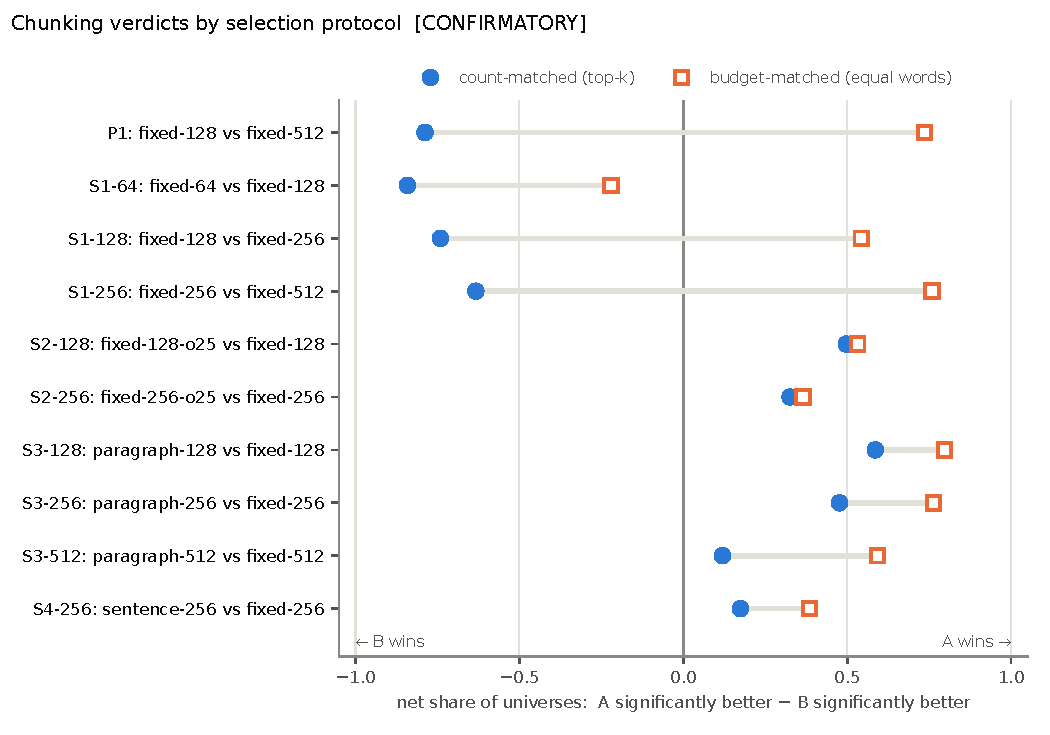
\includegraphics[width=0.94\linewidth]{figures/verdict_dumbbell.pdf}
\caption{Study 1 net support shares, $s_P(A)-s_P(B)$, for selected contrasts on the confirmatory split. Circles show count matching; open squares show word-budget matching. Movement to the right favors A relative to B, but need not reverse the favored arm.}
\label{fig:study1}
\end{figure}
% Generated by manuscript/make_tables.py from logged results. Do not edit by hand.
\begin{table*}[t]\centering\footnotesize
\caption{Study~1: share of universes (\%) whose 95\% paired-bootstrap CI supports arm A or arm B, per claim and selection protocol (confirmatory split); the remainder is inconclusive. Budget-matched universes use the admissible budgets $B \ge$ the larger chunk size. $n$ = number of universes.}\label{tab:e1claims}
\begin{tabular}{@{}lllrrrrrr@{}}\toprule
Claim & Role & A vs B & A (count) & B (count) & $n$ & A (budget) & B (budget) & $n$\\\midrule
P1 & primary & \texttt{fixed-128} vs \texttt{fixed-512} & 0.0 & 78.8 & 768 & 81.2 & 7.6 & 576\\
\midrule
S1-64 & secondary & \texttt{fixed-64} vs \texttt{fixed-128} & 0.0 & 84.1 & 768 & 20.0 & 42.1 & 960\\
S1-128 & secondary & \texttt{fixed-128} vs \texttt{fixed-256} & 0.0 & 74.1 & 768 & 60.5 & 6.2 & 768\\
S1-256 & secondary & \texttt{fixed-256} vs \texttt{fixed-512} & 0.0 & 63.3 & 768 & 78.0 & 2.1 & 576\\
\midrule
S2-64 & secondary & \texttt{fixed-64-o25} vs \texttt{fixed-64} & 52.5 & 1.7 & 768 & 54.8 & 1.8 & 960\\
S2-128 & secondary & \texttt{fixed-128-o25} vs \texttt{fixed-128} & 51.6 & 1.8 & 768 & 55.1 & 1.9 & 960\\
S2-256 & secondary & \texttt{fixed-256-o25} vs \texttt{fixed-256} & 36.1 & 3.5 & 768 & 39.8 & 3.3 & 768\\
S2-512 & secondary & \texttt{fixed-512-o25} vs \texttt{fixed-512} & 9.5 & 9.0 & 768 & 11.8 & 6.8 & 576\\
\midrule
S3-64 & secondary & \texttt{paragraph-64} vs \texttt{fixed-64} & 62.2 & 5.7 & 768 & 75.5 & 0.0 & 960\\
S3-128 & secondary & \texttt{paragraph-128} vs \texttt{fixed-128} & 59.8 & 1.2 & 768 & 79.7 & 0.0 & 960\\
S3-256 & secondary & \texttt{paragraph-256} vs \texttt{fixed-256} & 50.1 & 2.5 & 768 & 76.8 & 0.5 & 768\\
S3-512 & secondary & \texttt{paragraph-512} vs \texttt{fixed-512} & 13.7 & 1.7 & 768 & 60.9 & 1.7 & 576\\
\midrule
S4-64 & exploratory & \texttt{sentence-64} vs \texttt{fixed-64} & 58.9 & 6.1 & 768 & 69.5 & 0.4 & 960\\
S4-128 & exploratory & \texttt{sentence-128} vs \texttt{fixed-128} & 50.1 & 0.8 & 768 & 57.6 & 0.0 & 960\\
S4-256 & exploratory & \texttt{sentence-256} vs \texttt{fixed-256} & 19.0 & 1.6 & 768 & 38.5 & 0.0 & 768\\
S4-512 & exploratory & \texttt{sentence-512} vs \texttt{fixed-512} & 6.1 & 0.5 & 768 & 20.8 & 0.3 & 576\\
\bottomrule\end{tabular}
\end{table*}


The decline persists in all five sensitivity analyses: \SensBHEst\pp{} with multiplicity adjustment, \SensNoSquadEst\pp{} without SQuAD, \SensDefRetEst\pp{} with the default retriever, \SensClusterEst\pp{} with document-cluster resampling, and \SensAllBudgetsEst\pp{} with all budgets (Table~\ref{tab:e1sens}).

The mean P1 difference changes sign between protocols in each dataset (Table~\ref{tab:e1bydataset}). The strength of the change is not uniform. CUAD has relatively few decisive count-matched settings. Qasper has mixed budget-matched verdicts and only a small positive average difference. The coverage curves in Figure~\ref{fig:p1curve} show this variation rather than reducing it to a single pooled preference.
\begin{figure}[htbp]
\centering
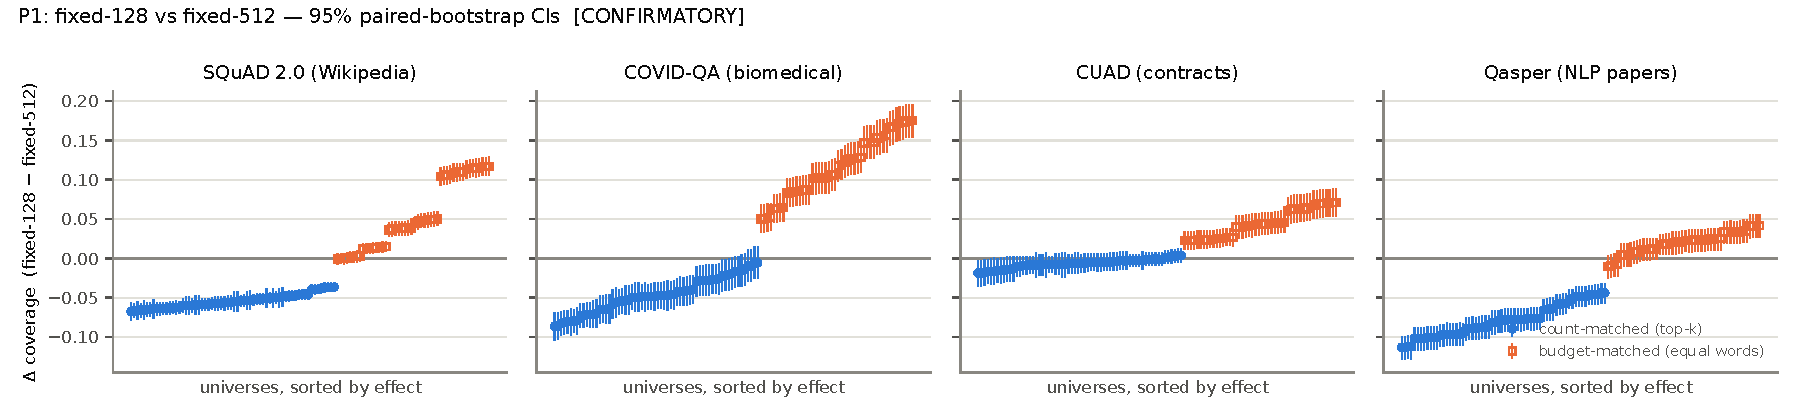
\includegraphics[width=\linewidth]{figures/speccurve_P1_coverage.pdf}
\caption{P1 coverage differences: \chunk{fixed-128} minus \chunk{fixed-512}, with 95\% paired-bootstrap intervals. Universes are sorted by effect within each dataset and distinguished by selection protocol.}
\label{fig:p1curve}
\end{figure}

\paragraph{Overlap, structure and size.}
Overlap comparisons change much less. For S2-128, overlap support moves from \StwoOneTwoEightCountA\% to \StwoOneTwoEightBudgetA\%; for S2-256, from \StwoTwoFiveSixCountA\% to \StwoTwoFiveSixBudgetA\%. These arms share a nominal cap, though terminal fragments produce slightly different mean lengths and overlap changes redundancy. Their relative stability supports the text-allowance explanation without isolating it from every other property of the retrieved context.

For S3-256, paragraph-packing support rises by \HOneBEst\pp{} (95\% CI [\HOneBLo, \HOneBHi]); H1b is \HOneBVerdict. Paragraph packing produces shorter chunks on average than fixed windows at the same cap. Budget matching removes the unequal allowance in word occurrences, while leaving differences in boundaries and ranking intact.

Smaller is not always better under budget matching. In S1-64, the 128-word arm retains \SoneSixFourBudgetB\% support, compared with \SoneSixFourBudgetA\% for the 64-word arm. The result is protocol dependence, not a rule to choose the smallest available chunk.

\paragraph{Dataset dependence and power.}
For S3-256 under budget matching, dataset has $\eta^2=\HTwoDatasetEta$, compared with \HTwoRetrieverEta{} for the retriever, and is the largest factor in \HTwoFraction\% of bootstrap replicates. H2 is \HTwoVerdict; the more precise decomposition is in Table~\ref{tab:e1h2}.

Across S2/S3 budget-matched universes, \HThreeShare\% have an estimated requirement above 500 paired queries, with median \HThreeMedianN{} (Table~\ref{tab:e1h3}). H3 is \HThreeVerdict. These estimates describe the observed paired-difference variance under the planning assumptions, not guaranteed power for a new document-clustered sample.

\begin{table}[tb]\centering\small
\caption{Pre-registered hypotheses and confirmatory outcomes. Share changes are percentage points, not retrieval-score improvements. H5b is a disclosed post-pilot amendment.}\label{tab:h}
\begin{tabular}{@{}llrll@{}}\toprule
ID & Quantity & Estimate & Interval or diagnostic & Verdict\\\midrule
H1 & Larger-arm decline, P1 & \HOneEst\pp & [\HOneLo, \HOneHi] & \HOneVerdict\\
H1b & Paragraph-256 gain & \HOneBEst\pp & [\HOneBLo, \HOneBHi] & \HOneBVerdict\\
H2 & Dataset main effect & $\eta^2=\HTwoDatasetEta$ & largest in \HTwoFraction\% & \HTwoVerdict\\
H3 & Universes needing $n>500$ & \HThreeShare\% & median $n=\HThreeMedianN$ & \HThreeVerdict\\\midrule
H4 & Shorter-arm gain, breakpoint & \HFourEst\pp & [\HFourLo, \HFourHi] & \HFourVerdict\\
H4b & Shorter-arm gain, clustering & \HFourBEst\pp & [\HFourBLo, \HFourBHi] & \HFourBVerdict\\
H5 & Larger-arm decline, dense P1 & \HFiveEst\pp & [\HFiveLo, \HFiveHi] & \HFiveVerdict\\
H5b & Shorter-arm gain, dense P1 & \HFiveBEst\pp & [\HFiveBLo, \HFiveBHi] & \HFiveBVerdict\\\bottomrule
\end{tabular}
\end{table}

\section{Study 1b: semantic chunking and dense retrieval}\label{sec:study1b}
\subsection{Design}
Study 1b extends the configurations while retaining the datasets, confirmatory queries, metrics and analysis procedure. It is not an independent replication on new data. Its pre-registration was frozen on 19 October 2026, after the exploratory pilot and before the confirmatory run.

\paragraph{Semantic chunkers.}
The \chunk{semantic-bp} arm embeds sentences individually and inserts a boundary when the cosine distance between adjacent sentences exceeds the document's 95th percentile, calculated with linear interpolation. A one-sentence document becomes one chunk. Overlong sentences are split first; groups exceeding 512 words are repacked with the sentence rule. The percentile is fixed in our design rather than attributed to Qu et al.'s evaluated settings.

The \chunk{semantic-cl} arm uses the positional--semantic distance introduced by Qu et al.~\cite{qu2025semanticchunking}:
\begin{align}
d(i,j)&=\lambda d_{\mathrm{pos}}(i,j)+(1-\lambda)d_{\mathrm{cos}}(i,j),\\
d_{\mathrm{pos}}(i,j)&=|i-j|/n,\qquad d_{\mathrm{cos}}(i,j)=1-\max\{\cos(e_i,e_j),0\}.
\end{align}
Here $n$ is the number of sentences and $e_i$ is a sentence embedding. We set $\lambda=0.5$, visit pairs with $d\leq0.5$ in increasing-distance order, break ties by sentence indices, and merge clusters only while their combined length remains at most 512 words. The resulting text can be non-contiguous; intervals are concatenated in document order. The word cap makes this an adaptation of the clustering procedure.

Both arms use the dense retriever's encoder. We compare each with \chunk{fixed-128}, \chunk{fixed-256} and \chunk{fixed-512}, denoting breakpoint contrasts S5 and clustering contrasts S6. Breakpoint chunks average \SemBpMin--\SemBpMax{} words across datasets, while clustering chunks average \SemClMin--\SemClMax{}. At least \SemClNoncontigMin\% of clustering chunks are non-contiguous (Table~\ref{tab:chunklen}). This setting produces clusters near the cap; it should not represent every possible semantic-clustering configuration.

\paragraph{Retrieval and hypotheses.}
We use default BM25 and BGE-M3 dense retrieval~\cite{chen2024bgem3}. Dense embeddings are normalized, stored in half precision and ranked by cosine similarity. The maximum encoder input is 8,192 tokens. Word caps and token counts are different quantities, so the cap alone is not a check for encoder truncation.

For each dataset and contrast, the shorter arm is determined from corpus-average chunk lengths computed before retrieval metrics. The breakpoint arm is longer than the 128- and 256-word fixed arms and shorter than the 512-word arm. Admissible budgets are 512, 1,024 and 2,048 words. Each S5/S6 contrast has \SfiveUniversesCount{} count-matched and \SfiveUniversesBudget{} budget-matched universes; dense-only P1 has \PoneDenseUniversesCount{} and \PoneDenseUniversesBudget{}, respectively.

H4 predicts a shorter-arm support gain of at least 20 percentage points across breakpoint contrasts and retrievers. H4b uses a 10-point threshold for clustering. H5 retains H1's larger-arm formulation under dense retrieval: a decline of at least 20 points in support for \chunk{fixed-512}.

The exploratory pilot showed that the larger arm was already infrequently supported with dense retrieval, limiting how far its share could fall. We therefore added H5b before the confirmatory run: a 20-point increase in support for the shorter arm. H5b changes the estimand and is reported as an amendment. H5 remains the original test.

\subsection{Results}
Across breakpoint comparisons, shorter-arm support rises from \HFourCount\% to \HFourBudget\%, a gain of \HFourEst\pp{} (95\% CI [\HFourLo, \HFourHi]). H4 is \HFourVerdict. The gain remains when retrievers are examined separately: \HFourBmOnlyEst\pp{} for BM25 and \HFourDenseOnlyEst\pp{} for dense retrieval. Table~\ref{tab:e3sens} reports the sensitivity analyses.

These shorter-arm shares should not be read as semantic-arm shares. Against \chunk{fixed-128}, the breakpoint arm is supported in \SfiveOneTwoEightCountSem\% of count-matched universes but only \SfiveOneTwoEightBudgetSem\% of budget-matched universes. Against \chunk{fixed-512}, where the breakpoint arm is shorter, its support increases instead (Table~\ref{tab:e3claims}). Relative length changes the interpretation of the same semantic-versus-fixed comparison.
\begin{figure}[htbp]
\centering
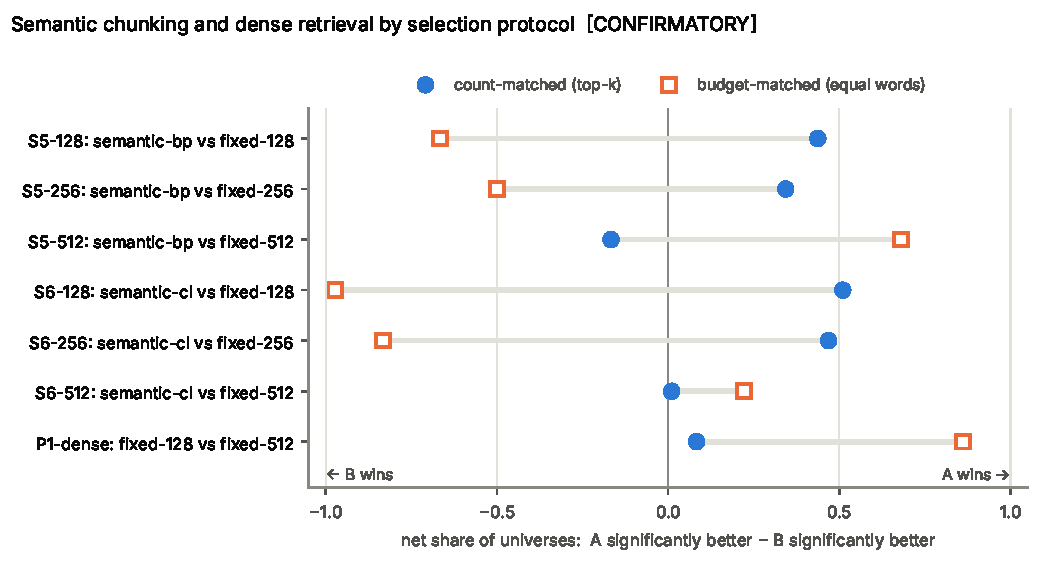
\includegraphics[width=0.95\linewidth]{figures/study1b_dumbbell.pdf}
\caption{Study 1b net support shares. S5/S6 pool default BM25 and dense retrieval; P1-dense uses only BGE-M3. A and B remain fixed within each row, so movement must be read alongside the pair's relative lengths.}
\label{fig:study1b}
\end{figure}
% Generated by manuscript/make_tables.py from logged results. Do not edit by hand.
\begin{table}[t]\centering\footnotesize
\caption{Study~1b: share of universes (\%) supporting arm A or B per claim and protocol (confirmatory). S5/S6 pool BM25 and dense retrieval; P1-dense uses the dense retriever only. Admissible budgets $B \in \{512, 1024, 2048\}$. The S5/S6 rows are the quantity reported by semantic-chunking studies (planned descriptive analysis g).}\label{tab:e3claims}
\begin{tabular}{@{}llrrrrrr@{}}\toprule
Claim & A vs B & A (count) & B (count) & $n$ & A (budget) & B (budget) & $n$\\\midrule
S5-128 & \texttt{semantic-bp} vs \texttt{fixed-128} & 60.4 & 16.7 & 96 & 8.3 & 75.0 & 72\\
S5-256 & \texttt{semantic-bp} vs \texttt{fixed-256} & 38.5 & 4.2 & 96 & 1.4 & 51.4 & 72\\
S5-512 & \texttt{semantic-bp} vs \texttt{fixed-512} & 7.3 & 24.0 & 96 & 68.1 & 0.0 & 72\\
\midrule
S6-128 & \texttt{semantic-cl} vs \texttt{fixed-128} & 53.1 & 2.1 & 96 & 0.0 & 97.2 & 72\\
S6-256 & \texttt{semantic-cl} vs \texttt{fixed-256} & 46.9 & 0.0 & 96 & 0.0 & 83.3 & 72\\
S6-512 & \texttt{semantic-cl} vs \texttt{fixed-512} & 18.8 & 17.7 & 96 & 33.3 & 11.1 & 72\\
\midrule
P1-dense & \texttt{fixed-128} vs \texttt{fixed-512} & 33.3 & 25.0 & 48 & 91.7 & 5.6 & 36\\
\bottomrule\end{tabular}
\end{table}


For clustering, shorter-arm support rises from \HFourBCount\% to \HFourBBudget\%, a gain of \HFourBEst\pp{} (95\% CI [\HFourBLo, \HFourBHi]). H4b is \HFourBVerdict{} for this configuration. The comparison does not separately identify effects of length, clustering and non-contiguity.

For dense P1, larger-arm support falls from \HFiveCountFiveTwelve\% to \HFiveBudgetFiveTwelve\%. The decline of \HFiveEst\pp{} (95\% CI [\HFiveLo, \HFiveHi]) is below the point-estimate threshold, while the interval extends above it. H5 is therefore \HFiveVerdict, even though the interval excludes zero. The amended shorter-arm share rises from \HFiveBCount\% to \HFiveBBudget\%, a gain of \HFiveBEst\pp{} ([\HFiveBLo, \HFiveBHi]); H5b is \HFiveBVerdict.

\section{Exploratory answer-quality evaluation}\label{sec:tier2}
\subsection{Setup}
We sampled 50 confirmatory queries per dataset using seed 20261019 and evaluated P1 and S3-256 with default BM25. The operating points were top-5 retrieval and a 1,024-word budget. The generation analysis plan was fixed before these runs; the check is exploratory and does not change any confirmatory hypothesis verdict.

The reader is Qwen3-4B~\cite{qwen2025qwen3}, using a Q4\_K\_M quantized GGUF model with greedy decoding, thinking disabled and a 256-token output limit. The prompt gives numbered passages and the question, requesting the shortest supported answer or exactly ``unanswerable''. We score answers by SQuAD-style token F1 and exact match. Model and prompt details are in Appendix~\ref{app:impl}.

For each query, let $\Delta_q(o)$ be the answer-score difference between A and B at operating point $o$. We estimate
\begin{equation}
\mathrm{DiD}_q=\Delta_q(B=1024)-\Delta_q(k=5).
\label{eq:did}
\end{equation}
A positive difference-in-differences (DiD) means that A gains relative to B when the protocol changes; it need not mean A has the higher score at either operating point. The pooled estimate weights datasets equally and uses 2,000 stratified bootstrap resamples. We compute the same contrast for retrieval coverage and report minimum detectable effects (MDEs).

\subsection{Results}
All scheduled generations completed. Coverage DiD is \EtwoPoneCov{} (95\% CI [\EtwoPoneCovLo, \EtwoPoneCovHi]) for P1 and \EtwoSthreeCov{} ([\EtwoSthreeCovLo, \EtwoSthreeCovHi]) for S3-256. Both contrasts are positive, consistent with the retrieval studies.

Answer F1 does not show the corresponding positive interaction. The pooled DiDs are \EtwoPoneFone{} ([\EtwoPoneFoneLo, \EtwoPoneFoneHi]) and \EtwoSthreeFone{} ([\EtwoSthreeFoneLo, \EtwoSthreeFoneHi]); both intervals include zero. This leaves the answer-F1 interaction unresolved rather than establishing equivalence.

For P1, exact match moves in the opposite direction: \EtwoPoneEm{} ([\EtwoPoneEmLo, \EtwoPoneEmHi]). The pooled cell means show the 128-word arm ahead at top-5 (\EtwoEmOneTwoEightCount{} versus \EtwoEmFiveTwelveCount), but the 512-word arm ahead at the matched budget (\EtwoEmFiveTwelveBudget{} versus \EtwoEmOneTwoEightBudget). These cell means are descriptive and have no separately reported intervals. Table~\ref{tab:e2did} gives the full contrasts.
% Generated by manuscript/make_tables.py from logged results. Do not edit by hand.
\begin{table*}[t]\centering\footnotesize
\caption{Answer-quality check (exploratory; written analysis plan\artifactref{experiments/E2_generation/ANALYSIS_PLAN.md}): difference-in-differences DiD $= \Delta(B{=}1{,}024) - \Delta(k{=}5)$, $\Delta$ = metric(A) $-$ metric(B), with 95\% bootstrap CIs (2{,}000 resamples; pooled: stratified by dataset). The retrieval mechanism predicts DiD $> 0$; an interval that includes 0 does not establish the absence of an effect. 50 queries per dataset; reader Qwen3-4B (Q4\_K\_M, greedy).}\label{tab:e2did}
\begin{tabular}{@{}llrrr@{}}\toprule
Claim & Dataset & Answer F1 & Exact match & Coverage\\\midrule
P1 & SQuAD 2.0 & $-$0.122 [$-$0.245, +0.009] & $-$0.160 [$-$0.300, 0.000] & +0.120 [+0.040, +0.220]\\
 & COVID-QA & $-$0.006 [$-$0.101, +0.090] & $-$0.060 [$-$0.160, +0.020] & +0.110 [+0.040, +0.200]\\
 & CUAD & $-$0.001 [$-$0.031, +0.033] & 0.000 [0.000, 0.000] & +0.020 [0.000, +0.060]\\
 & Qasper & +0.060 [$-$0.015, +0.158] & 0.000 [$-$0.060, +0.060] & +0.106 [+0.020, +0.214]\\
 & Pooled (stratified) & $-$0.017 [$-$0.065, +0.033] & $-$0.055 [$-$0.100, $-$0.010] & +0.089 [+0.050, +0.132]\\
 & Minimum detectable effect & 0.068 & 0.066 & 0.059\\
\midrule
S3-256 & SQuAD 2.0 & $-$0.027 [$-$0.104, +0.049] & $-$0.060 [$-$0.160, +0.060] & +0.060 [0.000, +0.140]\\
 & COVID-QA & +0.005 [$-$0.050, +0.066] & $-$0.020 [$-$0.100, +0.040] & +0.060 [0.000, +0.140]\\
 & CUAD & $-$0.008 [$-$0.027, +0.012] & 0.000 [0.000, 0.000] & 0.000 [0.000, 0.000]\\
 & Qasper & +0.045 [$-$0.017, +0.117] & +0.020 [0.000, +0.060] & +0.020 [0.000, +0.060]\\
 & Pooled (stratified) & +0.004 [$-$0.024, +0.036] & $-$0.015 [$-$0.050, +0.020] & +0.035 [+0.015, +0.060]\\
 & Minimum detectable effect & 0.044 & 0.051 & 0.036\\
\bottomrule\end{tabular}
\end{table*}


The P1 F1 MDE is \EtwoPoneFoneMde. An MDE describes statistical sensitivity under a power calculation; it is not an observed bound that excludes larger effects. The confidence intervals are the basis for interpreting this experiment.

Output length also matters. \EtwoTruncCuad{} of \EtwoJobsCuad{} CUAD outputs and \EtwoTruncQasper{} of \EtwoJobsQasper{} Qasper outputs reached the generation cap (Table~\ref{tab:e2diag}). The cap may affect scores for long answers, but we did not isolate that effect. An additional exploratory observation concerns SQuAD at the matched budget: F1 is \EtwoSquadFiveTwelveBudgetFone{} with the longer passages and \EtwoSquadOneTwoEightBudgetFone{} with the shorter passages, at similar coverage (\EtwoSquadFiveTwelveBudgetCov{} and \EtwoSquadOneTwoEightBudgetCov{}). Passage continuity is a possible explanation, not an established mechanism.

\section{A provisional audit of chunking evaluations}\label{sec:audit}
The protocol audit covers \AuditN{} empirical chunking studies published or posted in 2024--2026. Candidates were identified through logged web searches. Inclusion requires a comparison of at least two chunkings on a retrieval or answer metric and a conclusion about that comparison. The candidate list, coding protocol and conventions are maintained in \path{literature/protocol_audit/}.

We code the headline comparison's selection protocol, whether arm lengths differ, whether retrieved text volume is reported, whether uncertainty accompanies the chunking contrast, and the metric type. The exposure rule identifies count-based comparisons between unequal-length arms. It includes one reciprocal-rank comparison coded as ``other'', rather than fixed-$k$, under the recorded convention.

The coding contains \AuditFixedK{} fixed-count studies, \AuditBudget{} budget-matched study and \AuditUncertainty{} studies reporting a confidence interval or significance test for a chunking contrast. \AuditExposed{} entries are classified as exposed; one reports retrieved text volume. The complete coding appears in Table~\ref{tab:audit}.

The audit remains single-coded, with independent reliability assessment pending. Its exposed share is \AuditExposedPct\% (Wilson interval [\AuditExposedLo, \AuditExposedHi]\%), but this interval does not account for coding error or the non-probability selection of papers. We therefore use the audit as context, not as a prevalence estimate or evidence that the included papers' conclusions are wrong. Establishing exposure also requires attention to the metric: precision-sensitive evaluation is not interchangeable with the coverage metrics studied here.

\section{Discussion}\label{sec:discussion}
\subsection{What changes when the protocol changes?}
Count matching makes retrieval depth equal; budget matching makes the allowance in word occurrences equal. Neither holds every property of the context fixed. Longer passages may contain more evidence, but segmentation also affects ranking, redundancy, boundaries and continuity. The small overlap shifts and the direction of the unequal-length comparisons are consistent with text allowance contributing to protocol sensitivity. They do not identify it as the sole cause.

Budget matching also has costs. It can cut through the final passage, and equal word counts do not imply equal model-token counts, unique context, indexing cost or latency. These are reasons to specify the constraint, not reasons to avoid the comparison. Fixed-$k$ evaluation answers a legitimate deployment question when the system retrieves a fixed number of passages. The problem arises when its answer is presented as an intrinsic property of a chunker.

\subsection{Why retrieval evidence is not enough}
The dense retriever begins with a different preference from the lexical grid: larger fixed chunks are less dominant even under count matching. Topic mixing within an embedding is one possible explanation, but our experiment does not measure that mechanism. What it establishes is configuration dependence.

The answer experiment adds a second distinction. Increased gold-span coverage can coexist with unresolved answer-F1 effects and an exact-match interaction in the opposite direction. A reader may respond differently to passage continuity, distractors, answer length and normalization. The present check cannot separate those explanations, and its single-reader setting does not support a general claim that protocol effects stop at retrieval.

\subsection{Reporting implications}
A chunking comparison should specify nominal caps, realized length distributions, overlap handling, retriever, metric and operating point. For the retrieved context, it should report both passage count and word or token volume, including the treatment of repeated text and the final chunk. Showing count-matched and budget-matched results side by side makes their different constraints visible.

Statistical summaries need the same precision. Support shares require universe counts, grid weights and an uncertainty procedure. They should not be called flip rates without pairing universes and measuring transitions. Query-level and document-level resampling should be distinguished. Finally, retrieval and answer outcomes should be reported separately: neither substitutes for the other.

\section{Limitations and threats to validity}\label{sec:limitations}
\paragraph{Measurement.}
Our span metrics reward any qualifying or best-covered evidence span and do not penalize irrelevant context. They need not predict precision, complete multi-hop evidence acquisition, factuality or answer quality. Word budgets count repeated occurrences, whereas coverage is measured on unique character positions.

\paragraph{Implementation and scope.}
Sentence splitting is rule-based, paragraph boundaries depend on blank lines, and budget selection can truncate a chunk. Each semantic chunker uses one setting. The clustering arm is mostly non-contiguous and close to its cap. Same-cap overlap contrasts differ in realized lengths and redundancy, so they are not exact mechanistic controls. The study covers four English collections, one lexical family and one dense encoder. Study 1b reuses Study 1's confirmatory queries. The answer check uses one quantized reader, a small query sample and an output cap that truncated some responses.

\paragraph{Inference.}
Universes are correlated settings, not independent replications. Joint query resampling preserves their shared-query dependence but does not sample new datasets; document dependence is addressed by a sensitivity analysis. Support shares depend on the grid, its weights and the significance rule. H3 uses an approximate power calculation. The answer experiment is exploratory, not a multiplicity-controlled family of confirmatory tests.

\paragraph{Study history and audit.}
H5b was added after the exploratory pilot and before confirmatory evaluation. A document-bootstrap sensitivity interval was corrected after the Study 1 run. Both changes remain explicit in Appendix~\ref{app:deviations}. The literature audit has not completed independent double-coding and should not support a definitive claim about the prevalence of protocol-related problems.

\section{Conclusion}
Chunking verdicts depend on the retrieval-selection protocol. Matching words instead of chunk count reduces support for the larger fixed arm by \HOneEst\pp{} in the primary lexical comparison. In breakpoint comparisons, the shorter arm gains \HFourEst\pp{}. These are changes in support shares within the evaluated grid, not universal rankings of chunkers. The original dense-retrieval hypothesis remains inconclusive, while its disclosed shorter-arm amendment is supported.

The answer-quality check does not establish a corresponding positive F1 interaction. The practical lesson is to state what the comparison holds constant: report retrieval depth and text budget, and test answer quality rather than infer it from evidence coverage.

\section{Reproducibility}\label{sec:reproducibility}
The research repository is available at \\url{https://github.com/swaroopchandrashekar13/rag-research}. It records the pre-registrations, deviation logs, dataset manifests, run configurations and analysis outputs. Numerical results in the text and hypothesis summary use macros generated by \\path{manuscript/make_numbers.py}; the detailed result tables are included directly from the outputs of \\path{manuscript/make_tables.py}. Re-running these scripts after an analysis update keeps the manuscript linked to the results. Bibliographic keys are maintained in \\path{refs.bib}.


\FloatBarrier
\bibliographystyle{plainnat}
\bibliography{refs}

\clearpage
\appendix
\section{Deviations from the pre-registrations}\label{app:deviations}
Table~\ref{tab:deviations} summarizes the logged changes in the two pre-registration documents. H5b adds a secondary hypothesis without replacing H5. The post-run Study 1 correction changes the document-cluster sensitivity interval, not its point estimate or verdict.
\begin{table}[htbp]\centering\footnotesize
\caption{Study-plan deviations and their timing.}\label{tab:deviations}
\begin{tabular}{@{}>{\raggedright\arraybackslash}p{1.55cm}>{\raggedright\arraybackslash}p{5.5cm}>{\raggedright\arraybackslash}p{7.4cm}@{}}\toprule
Study & Change & Timing and consequence\\\midrule
Study 1 & Restrict main budgets to $B\geq\max(W_A,W_B)$; retain all budgets for sensitivity analysis & Before the pilot and confirmatory run; a smoke test showed that smaller budgets force truncation of the first chunk.\\
Study 1 & Add document-cluster resampling & Before the runs; multiple queries are nested in a small number of SQuAD articles.\\
Study 1 & Align the $\eta^2$ description with the analytic implementation & After the pilot and before freezing; the estimand and thresholds are unchanged.\\
Study 1 & Correct query-level resampling inside the document-cluster sensitivity interval & After the confirmatory run; the interval changes, while the point estimate and verdict do not.\\
Answer check & Replace the hosted reader with local Qwen3-4B; fix the sample and operating points & Before analyzed generation, following API-quota limits; the check remains exploratory.\\
Study 1b & Specify implementation details & During implementation, before pilot output.\\
Study 1b & Add H5b and retain H5 & After the exploratory pilot, before the confirmatory run; a new secondary estimand is disclosed.\\
Study 1b & Retain the clustering defaults despite near-cap chunks & After the pilot; the configuration is not tuned to improve the observed outcome.\\\bottomrule
\end{tabular}
\end{table}

\FloatBarrier
\section{Implementation details}\label{app:impl}
\paragraph{Dense retrieval.}
The run uses BGE-M3 revision \texttt{5617a9f61b02}, with \texttt{sentence-transformers} 6.1.0, \texttt{transformers} 5.20.1 and \texttt{torch} 2.14.1. Normalized embeddings are cached in half precision. Equal cosine scores are ordered by the lower chunk index. The Study 1b manifest identifies the run configuration and model revision; half-precision embeddings should not be assumed bit-identical across hardware.

\paragraph{Reader and prompt.}
The reader uses the Qwen3-4B GGUF Q4\_K\_M file at revision \texttt{bc640142}, with \texttt{llama-cpp-python} 0.3.36. The model-file SHA-256 is
\begin{quote}\ttfamily\small
7485fe6f\allowbreak11af2943\allowbreak3bc51cab\allowbreak58009521\allowbreak f205840f\allowbreak5b4ae3a3\allowbreak2fa7f92e\allowbreak8534fdf5.
\end{quote}
The ChatML prompt contains an empty thinking block. Decoding uses temperature zero, top-$k$ one, seed 7 and the 256-token cap. The system instruction is:
\begin{quote}\small
Answer the question using only the numbered passages. Reply with the shortest answer that is fully supported by the passages, copying the wording from them where possible. If the passages do not contain the answer, reply exactly: unanswerable
\end{quote}
The user message lists numbered passages, followed by the question and an answer cue. Keeping this wording fixed prevents prompt changes from being mixed into the protocol contrast.

\FloatBarrier
\section{Additional retrieval results}\label{app:retrieval}
The tables below give corpus-level chunk lengths, per-dataset results, sensitivity analyses and power calculations. Corpus mean length should be distinguished from the amount of text actually selected for a query.
% Generated by manuscript/make_tables.py from logged results. Do not edit by hand.
\begin{table}[t]\centering\small
\caption{Mean chunk length in words per chunking and dataset (full retrieval corpus), from the run manifests; they depend only on the chunking, not on any retrieval metric. These lengths define the ``shorter arm'' of every Study~1b claim. The fixed chunkings of Study~1b are the same chunks as in Study~1.}\label{tab:chunklen}
\begin{tabular}{@{}lrrrr@{}}\toprule
Chunking & SQuAD 2.0 & COVID-QA & CUAD & Qasper\\\midrule
\texttt{fixed-64} & 64 & 64 & 64 & 63\\
\texttt{fixed-128} & 126 & 126 & 127 & 126\\
\texttt{fixed-256} & 249 & 247 & 252 & 247\\
\texttt{fixed-512} & 485 & 483 & 495 & 477\\
\texttt{fixed-64-o25} & 64 & 64 & 64 & 64\\
\texttt{fixed-128-o25} & 127 & 127 & 127 & 127\\
\texttt{fixed-256-o25} & 252 & 252 & 253 & 251\\
\texttt{fixed-512-o25} & 497 & 494 & 502 & 491\\
\texttt{sentence-64} & 49 & 49 & 46 & 50\\
\texttt{sentence-128} & 111 & 111 & 98 & 113\\
\texttt{sentence-256} & 235 & 234 & 213 & 235\\
\texttt{sentence-512} & 476 & 470 & 453 & 466\\
\texttt{paragraph-64} & 46 & 45 & 41 & 42\\
\texttt{paragraph-128} & 90 & 90 & 85 & 88\\
\texttt{paragraph-256} & 187 & 179 & 174 & 199\\
\texttt{paragraph-512} & 420 & 392 & 379 & 435\\
\midrule
\texttt{semantic-bp} & 293 & 287 & 320 & 278\\
\texttt{semantic-cl} & 456 & 455 & 458 & 452\\
\quad non-contiguous chunks (\%) & 92.5 & 94.1 & 92.0 & 94.7\\
\bottomrule\end{tabular}
\end{table}

% Generated by manuscript/make_tables.py from logged results. Do not edit by hand.
\begin{table}[t]\centering\footnotesize
\caption{Study~1 per dataset: share of universes (\%) supporting arm A or B, and the mean difference $\bar\Delta = $ metric(A) $-$ metric(B) over universes. P1: A = fixed-128, B = fixed-512. S3-256: A = paragraph-256, B = fixed-256.}\label{tab:e1bydataset}
\begin{tabular}{@{}llrrrrrr@{}}\toprule
Claim & Dataset & A (count) & B (count) & $\bar\Delta$ (count) & A (budget) & B (budget) & $\bar\Delta$ (budget)\\\midrule
P1 & SQuAD 2.0 & 0.0 & 100.0 & $-$0.055 & 83.3 & 0.0 & +0.053\\
 & COVID-QA & 0.0 & 89.1 & $-$0.054 & 100.0 & 0.0 & +0.109\\
 & CUAD & 0.0 & 26.0 & $-$0.009 & 97.2 & 0.0 & +0.040\\
 & Qasper & 0.0 & 100.0 & $-$0.093 & 44.4 & 30.6 & +0.002\\
\midrule
S3-256 & SQuAD 2.0 & 69.3 & 0.0 & +0.014 & 100.0 & 0.0 & +0.034\\
 & COVID-QA & 77.1 & 0.0 & +0.028 & 100.0 & 0.0 & +0.058\\
 & CUAD & 1.0 & 9.9 & $-$0.003 & 8.3 & 2.1 & +0.002\\
 & Qasper & 53.1 & 0.0 & +0.019 & 99.0 & 0.0 & +0.030\\
\bottomrule\end{tabular}
\end{table}

% Generated by manuscript/make_tables.py from logged results. Do not edit by hand.
\begin{table}[t]\centering\small
\caption{Study~1, H1 under the planned sensitivity analyses: drop in the share of universes supporting fixed-512 from count- to budget-matched selection, in percentage points (threshold 20). (a) changes the verdict rule and has no joint-bootstrap CI.}\label{tab:e1sens}
\begin{tabular}{@{}lrl@{}}\toprule
Analysis & Estimate (pp) & 95\% CI\\\midrule
Main analysis (as planned) & 71.1 & [64.8, 81.9]\\
\midrule
(a) Benjamini--Hochberg FDR 5\% within claim, protocol and dataset & 68.0 & ---\\
(b) without SQuAD 2.0 & 61.5 & [53.2, 74.8]\\
(c) default retriever only (Lucene, $k_1$=1.5, $b$=0.75, stemmed) & 70.8 & [64.6, 85.4]\\
(d) document-cluster bootstrap & 69.7 & [63.8, 82.0]\\
(e) all budgets, including $B <$ chunk size & 74.2 & [68.3, 84.8]\\
\bottomrule\end{tabular}
\end{table}

% Generated by manuscript/make_tables.py from logged results. Do not edit by hand.
\begin{table}[t]\centering\small
\caption{Study~1, H2: main-effects decomposition of $\Delta_u$ for S3-256 under budget-matched selection.}\label{tab:e1h2}
\begin{tabular}{@{}lr@{}}\toprule
Quantity & Value\\\midrule
$\eta^2$ of dataset & 0.614\\
$\eta^2$ of budget & 0.096\\
$\eta^2$ of retriever & 0.044\\
$\eta^2$ of metric & 0.032\\
dataset largest (share of bootstrap replicates) & 100.0\%\\
\bottomrule\end{tabular}
\end{table}

% Generated by manuscript/make_tables.py from logged results. Do not edit by hand.
\begin{table}[t]\centering\small
\caption{Study~1, H3: paired queries needed to detect $|\delta| = 0.02$ ($\alpha=0.05$ two-sided, power 0.8), $n = ((1.96 + 0.8416)\,\sigma_d / 0.02)^2$, per budget-matched universe.}\label{tab:e1h3}
\begin{tabular}{@{}lrr@{}}\toprule
Claim & Median $n$ & Universes with $n > 500$ (\%)\\\midrule
S2-64 & 1,175 & 82.5\\
S2-128 & 1,162 & 84.8\\
S2-256 & 1,149 & 79.7\\
S2-512 & 1,161 & 78.0\\
S3-64 & 1,498 & 92.5\\
S3-128 & 1,412 & 90.6\\
S3-256 & 1,399 & 86.2\\
S3-512 & 1,248 & 84.7\\
\midrule
All S2 and S3 universes & 1,256 & 85.4\\
\bottomrule\end{tabular}
\end{table}

% Generated by manuscript/make_tables.py from logged results. Do not edit by hand.
\begin{table}[t]\centering\small
\caption{Study~1b, H4 under the planned sensitivity analyses: share of S5 universes (\%) supporting the shorter arm under count- and budget-matched selection, and the difference (pp; threshold 20). Study~1b uses only the default BM25 configuration, so sensitivity (c), the default-retriever restriction, does not apply.}\label{tab:e3sens}
\begin{tabular}{@{}lrrrl@{}}\toprule
Analysis & Count & Budget & Difference & 95\% CI\\\midrule
Main analysis (H4 as planned) & 9.4 & 64.8 & 55.4 & [50.8, 63.1]\\
\midrule
(a) Benjamini--Hochberg FDR 5\% within claim, protocol and dataset & --- & --- & 54.3 & ---\\
(b) without SQuAD 2.0 & 6.9 & 54.9 & 48.0 & [42.7, 58.3]\\
(d) document-cluster bootstrap & 8.0 & 66.7 & 58.7 & [50.0, 63.3]\\
(e) all budgets & 9.4 & 63.1 & 53.7 & [49.7, 60.9]\\
(f) BM25 only & 0.0 & 61.1 & 61.1 & [57.2, 72.5]\\
(f) dense only & 18.8 & 68.5 & 49.8 & [39.1, 58.1]\\
\bottomrule\end{tabular}
\end{table}

\begin{figure}[htbp]
\centering
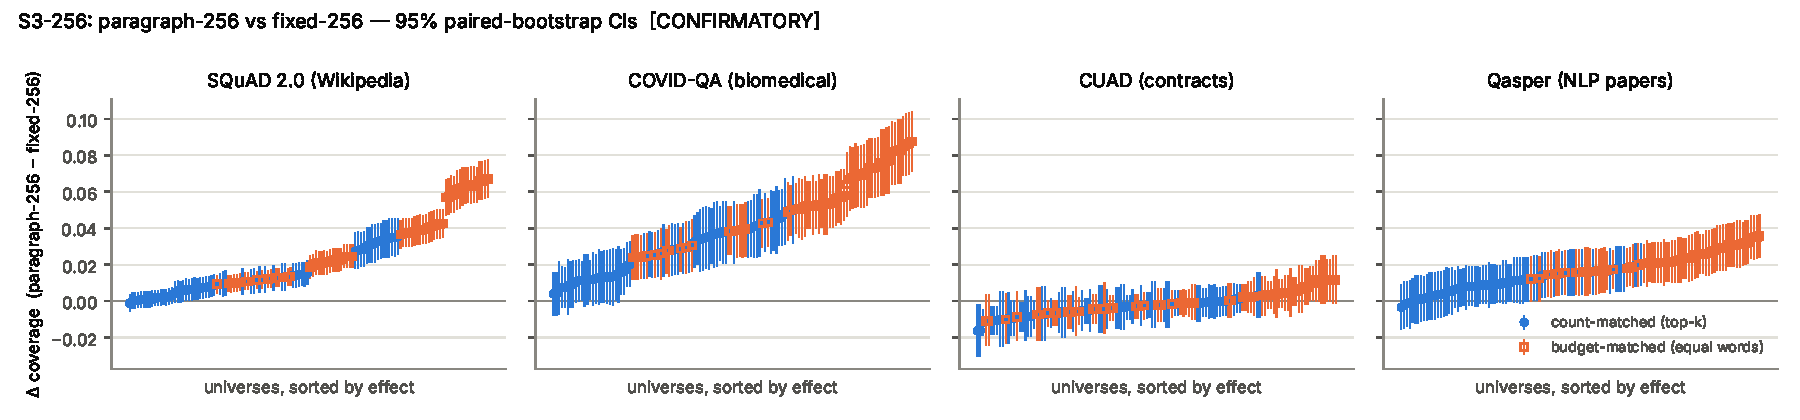
\includegraphics[width=\linewidth]{figures/speccurve_S3-256_coverage.pdf}
\caption{S3-256 coverage differences: paragraph packing minus fixed windows at a 256-word cap, with 95\% paired-bootstrap intervals. Universes are sorted by effect within each dataset. The near-zero CUAD effects show that the paragraph-packing result is not uniform across domains.}
\label{fig:s3curve}
\end{figure}

\FloatBarrier
\section{Generation diagnostics}\label{app:diagnostics}
Table~\ref{tab:e2diag} summarizes completion, truncation and answer behavior across the repeated arm-by-protocol generations. The correlation is descriptive, not causal. A lenient hit means that at least half of one gold span was retrieved; it does not mean that all required evidence was present.
% Generated by manuscript/make_tables.py from logged results. Do not edit by hand.
\begin{table}[t]\centering\footnotesize
\caption{Answer-quality check, planned diagnostics per dataset (400 generations each): completed jobs, answers truncated at the 256-token cap, share of ``unanswerable'' replies, and the link between retrieval and answers (Pearson correlation of coverage and F1; mean F1 when the gold evidence was / was not at least half retrieved).}\label{tab:e2diag}
\begin{tabular}{@{}lrrrrrr@{}}\toprule
Dataset & Jobs ok & Truncated & Unanswerable (\%) & $r$(coverage, F1) & F1 | hit & F1 | miss\\\midrule
SQuAD 2.0 & 400/400 & 0 & 4.2 & 0.36 & 0.56 & 0.06\\
COVID-QA & 400/400 & 0 & 5.8 & 0.33 & 0.40 & 0.15\\
CUAD & 400/400 & 65 & 15.0 & 0.66 & 0.70 & 0.14\\
Qasper & 400/400 & 2 & 15.8 & 0.53 & 0.37 & 0.08\\
\bottomrule\end{tabular}
\end{table}


\clearpage
\section{Protocol-audit records}\label{app:audit}
Table~\ref{tab:audit} retains the recorded classifications, including ``other'', ``unclear'' and ``possibly exposed''. The cited publications identify the records being coded. Bibliographic verification does not establish the reliability of those protocol codes; the audit remains provisional until independent coding is complete.
% Generated by manuscript/make_tables.py from logged results. Do not edit by hand.
\begin{table*}[t]\centering\footnotesize
\caption{Protocol audit: coding of each included study (provisional; see Section~\ref{sec:audit}). Protocol: how arms are compared; Length differs: whether the compared arms produce chunks of different length; Text reported: whether the amount of retrieved text is reported; Uncertainty: for chunking contrasts; Exposure: derived by the audit's coding rules\artifactref{literature/protocol_audit/analyze_audit.py}.}\label{tab:audit}
\begin{tabular}{@{}lllllll@{}}\toprule
Study & Protocol & Length differs & Text reported & Uncertainty & Metric & Exposure\\\midrule
\citeL{qu2025semanticchunking} & fixed $k$ & unclear & no & none & both & possibly exposed\\
\citeL{bhat2025chunksize} & fixed $k$ & yes & no & none & retrieval & exposed\\
\citeL{muthyam2026ragstability} & fixed $k$ & yes & yes & seeds & both & exposed, text reported\\
\citeL{beyondchunkthenembed2026} & fixed $k$ & yes & no & test & retrieval & exposed\\
\citeL{chunkembedsensitivity2026} & fixed $k$ & yes & no & CI & retrieval & exposed\\
\citeL{garrido2026chunksize} & other & yes & no & none & retrieval & exposed\\
\citeL{chunkingcost2026} & fixed $k$ & yes & no & none & both & exposed\\
\citeL{pdfparsingfin2026} & other & unclear & no & none & both & not exposed\\
\citeL{chunkingacademic2026} & unclear & unclear & no & none & both & undeterminable\\
\citeL{reconstructingcontext2025} & other & unclear & no & none & both & not exposed\\
\citeL{hichunk2025} & budget & yes & yes & none & both & not exposed\\
\citeL{metachunking2024} & fixed $k$ & no & no & none & answer & not exposed\\
\citeL{freechunker2025} & fixed $k$ & unclear & no & seeds & answer & possibly exposed\\
\citeL{moc2025} & fixed $k$ & no & no & CI & answer & not exposed\\
\citeL{queryadaptivechunking2026} & fixed $k$ & yes & no & seeds & both & exposed\\
\citeL{arabicrag2025} & unclear & unclear & no & none & both & undeterminable\\
\citeL{jimenoyepes2024financial} & fixed $k$ & yes & no & none & both & exposed\\
\citeL{duarte2024lumberchunker} & fixed $k$ & yes & no & none & both & exposed\\
\citeL{gunther2024latechunking} & other & no & no & none & retrieval & not exposed\\
\bottomrule\end{tabular}
\end{table*}

\FloatBarrier
\end{document}